\documentclass{amsart}
\usepackage{amssymb,
enumitem,
mathrsfs,
hyperref,
tikz,
upgreek,
subcaption,
graphics
}
\usetikzlibrary{decorations.pathreplacing}
\usepackage[T1]{fontenc}
\usepackage[utf8]{inputenc}

\newcommand{\ball}[2]{\shade[ball color=black!30!white] (#1,#2,0) circle (.3cm)}

\begin{document}

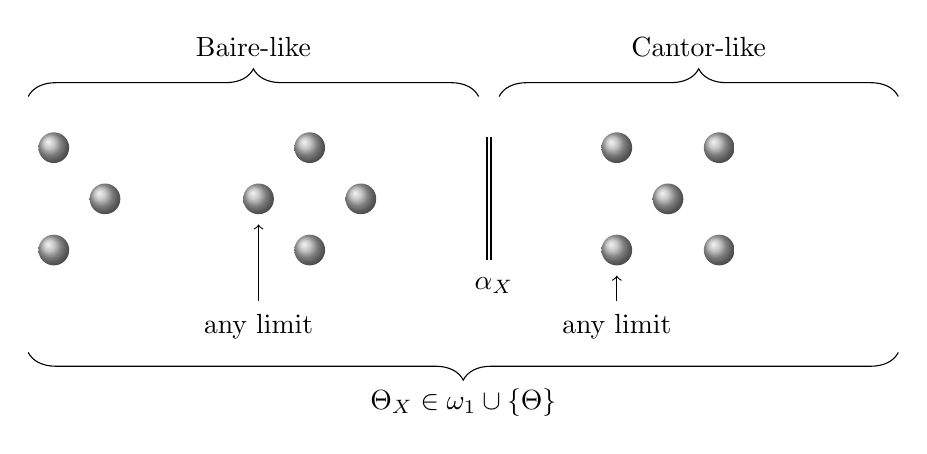
\begin{tikzpicture}[scale=0.65]
\ball{0}{1};
\ball{0}{-1};
\ball{1}{0};
\node at (2.5,0) {\( \dotsc \)};
\ball{4}{0};
\ball{5}{1};
\ball{5}{-1};
\ball{6}{0};
\node at (7.5,0) {\( \dotsc \)};
\draw [thick,double] (8.5,1.2)--(8.5,-1.2);
\node at (9.5,0) {\( \dotsc \)};
\ball{11}{1};
\ball{11}{-1};
\ball{12}{0};
\ball{13}{1};
\ball{13}{-1};
\node at (14.5,0) {\( \dotsc \)};
\node at (4,-2.5) {any limit};
\draw [->] (4,-2)--(4, -0.5);
\node at (11,-2.5) {any limit};
\draw [->] (11,-2)--(11, -1.5);
\node at (8.6,-1.7) {\( \alpha_X \)};
\draw [decorate,decoration={brace,mirror,amplitude=10pt}]
    (-0.5,-3) -- (16.5,-3) node [midway,yshift=-0.25in] {\( \Theta_{X} \in \omega_1 \cup \{ \Theta \} \)};
    \draw [decorate,decoration={brace,amplitude=10pt}]
    (-0.5,2) -- (8.3,2) node [midway,yshift=0.25in] {Baire-like};
        \draw [decorate,decoration={brace,amplitude=10pt}]
    (8.7,2) -- (16.5,2) node [midway,yshift=0.25in] {Cantor-like};
\end{tikzpicture}

\end{document}